\chapter{Introdução}

O presente trabalho detalha as atividades desenvolvidas durante o estágio obrigatório na empresa LifesHub, em Florianópolis, no ano de 2025, focadas no desenvolvimento de um sistema de processamento de dados para o setor de saúde suplementar. O trabalho aborda a criação de um pipeline de Extração, Transformação e Carga (ETL), projetado para automatizar a coleta, o tratamento e o enriquecimento de grandes volumes de dados públicos. O problema central que norteia este projeto é a alta complexidade e a descentralização das fontes de dados de saúde no Brasil, um obstáculo que dificulta a geração de análises estratégicas e inteligência de mercado para os agentes do setor.

\section{Contextualização}

O cenário da saúde suplementar no Brasil é caracterizado por um ecossistema de dados vasto e diversificado, disponibilizado publicamente por diferentes órgãos governamentais. Fontes como a ANS, CNES e o DATASUS (com seus subsistemas SIH, SIA e CIHA) oferecem um volume massivo de informações sobre operadoras, beneficiários, estabelecimentos e procedimentos. No entanto, a extração de valor desses dados é um desafio significativo. As informações são descentralizadas, armazenadas em formatos heterogêneos — como arquivos de banco de dados (.dbc), planilhas (.xlsx) e texto (.csv) — e frequentemente exigem um complexo processo de limpeza, padronização e cruzamento para se tornarem úteis.

Nesse contexto, a LifesHub se posiciona como uma empresa de tecnologia especializada em resolver essa complexidade. A companhia atua na consolidação e no enriquecimento desses dados públicos, transformando-os em uma plataforma de inteligência de mercado para os diversos players do setor, como hospitais, operadoras de planos de saúde e indústria farmacêutica. O projeto desenvolvido neste estágio está diretamente inserido nessa missão, focando na construção da infraestrutura de engenharia de dados — o pipeline de ETL — responsável por automatizar e escalar a capacidade da empresa de processar e entregar dados de alta qualidade.
A arquitetura desta solução e as tecnologias empregadas serão detalhadas nos capítulos subsequentes.

\newpage
\section{Contexto na Engenharia de Controle e Automação}

O desenvolvimento deste projeto aplica diretamente os conceitos fundamentais da Engenharia de Controle e Automação, indo além de um simples processamento de dados para construir um sistema verdadeiramente autônomo. As conexões com a área são evidentes nos seguintes pilares:

\textbf{Automação e Controle Supervisório:} 

O sistema implementa um controle em malha aberta com supervisão automatizada. Um agente de software (bot) monitora continuamente as fontes de dados externas, como servidores FTP Ao identificar um evento, ele dispara a execução do pipeline de ETL correspondente, funcionando como um controlador que automatiza todo o fluxo de trabalho sem intervenção humana.

\textbf{Integração de Sistemas:}

O projeto é um caso prático de integração de sistemas. A solução orquestra a comunicação entre tecnologias distintas, incluindo servidores FTP, a plataforma de armazenamento em nuvem Azure Blob Storage e o motor de processamento em memória DuckDB.

\textbf{Programação e Desenvolvimento de Sistemas:}

A implementação da lógica foi realizada em Python, seguindo uma arquitetura modular com responsabilidades bem definidas entre orquestração, execução e configuração, aplicando os princípios de desenvolvimento de sistemas automatizados.

\textbf{Análise de Dados para Otimização:}

O objetivo final do sistema automatizado é fornecer dados consistentes e atualizados que sirvam de base para a tomada de decisão estratégica. Ao garantir a disponibilidade de informações de alta qualidade, o projeto habilita a aplicação de técnicas de avaliação de desempenho, essencial para a otimização de processos no setor de saúde.

\section{Objetivos}

O principal objetivo deste projeto é o desenvolvimento de um pipeline de Etração, Transformação e Carga de dados. Os requisitos para que seja alcançado um bom resultado, é a robustez, escabilidade e automação do processo, focando no processamento de dados do setor de saúde suplementar no Brasil. A solução procura converter um grande volumes de dados públicos brutos, vindos de diferentes fontes em um ativo de dados estruturado e confiável e pronto para análise. Todo o sistema foi desenhado para garantir armazenamento e acessibilidade dos dados, agregando valor para os clientes da empresa.

Adicionalmente, era necessário que o sistema fosse escálavel e flexível, empregando tecnologias open-source como Python e DuckDB, integradas a infraestrutura de nuvem da Microsoft Azure. Toda a soluçaõ foi modularizada e configuarada, facilitando a implantação, manutenção e futuras modificações. Esta estrutura garante que o sistema possa ser estendida para novos casos de usos ou novas fontes de dados.

Foram definidos os seguintes objetivos:

\begin{itemize}
    \item Orquestrador de pipelines modular em Python para gerenciar a execução das tarefas, garantindo automação do fluxo de dados.
    \item Implementar o DuckDB como processamento analítico para gerenciar e transformar os dados brutos.
    \item Utilizar o sistema de Azure para servir como repositório centralizado. Armazenamento de dados brutos e processados.
\end{itemize}

\section{Metodologia}

Essa seção descreve as metodologias e princípios utilizados durante a realização do estágio na empresa. Essas práticas garantem uma colaboração organizada entre os os colaboradores durante diferentes fases de desenvolvimento.

\subsection{Framework Scrum}

Aplicamos a metodolgia ágil de gerenciamento de projetos SCRUM. Com ciclos curtos chamados sprints, entregamos valor de forma continua e adáptavel. As cerimônias foram adaptadas ao ritmo da equipe da seguinte forma.

\textbf{Planejamento e execução:} O trabalho foi organizado em ciclos de duas semanas. As tarefas desenvolvidas eram selecionadas através do backlog e movidas para a sprint no início de cada ciclo.

\textbf{Reuniões:} Todas as terças-feiras, a equipe realizava a weekly, para discutirmos o progresso das tarefas em andamentos, identificar impedintos e alinhas as prioridades para o resto da semana.

\textbf{Gerenciamento de tarefas e documentação:} A ferramenta Notion foi utilizada como plataforma de controle. Nela, eram mantidos os quadros de tarefas (cards), o backlog, e o registro de horas (log de horas) dedicado a cada atividade, garantindo o acompanhamento detalhado do processo de cada entrega.

\subsection{Versionamento de código}

O controle de versão do código-fonte do projeto foi realizado através do Git. A escolha dessa ferramenta foi fundamental para permitir o desenvolvimento paralelo de novas funcionalidades, correção de bugs de forma isolada e colaboração entre membros da equipe sem o risco de sobrescrever o trabalho.

A estratégia de ramificação, branching, permitiu o controle de novas implentações de forma contínua, após validades integradas ao código principal (main). Assim, garantindo estabilidade e integridade ao sistema.

\begin{figure}[H]
  \centering
  \caption{Git workflow}\label{fig:git_workflow}
  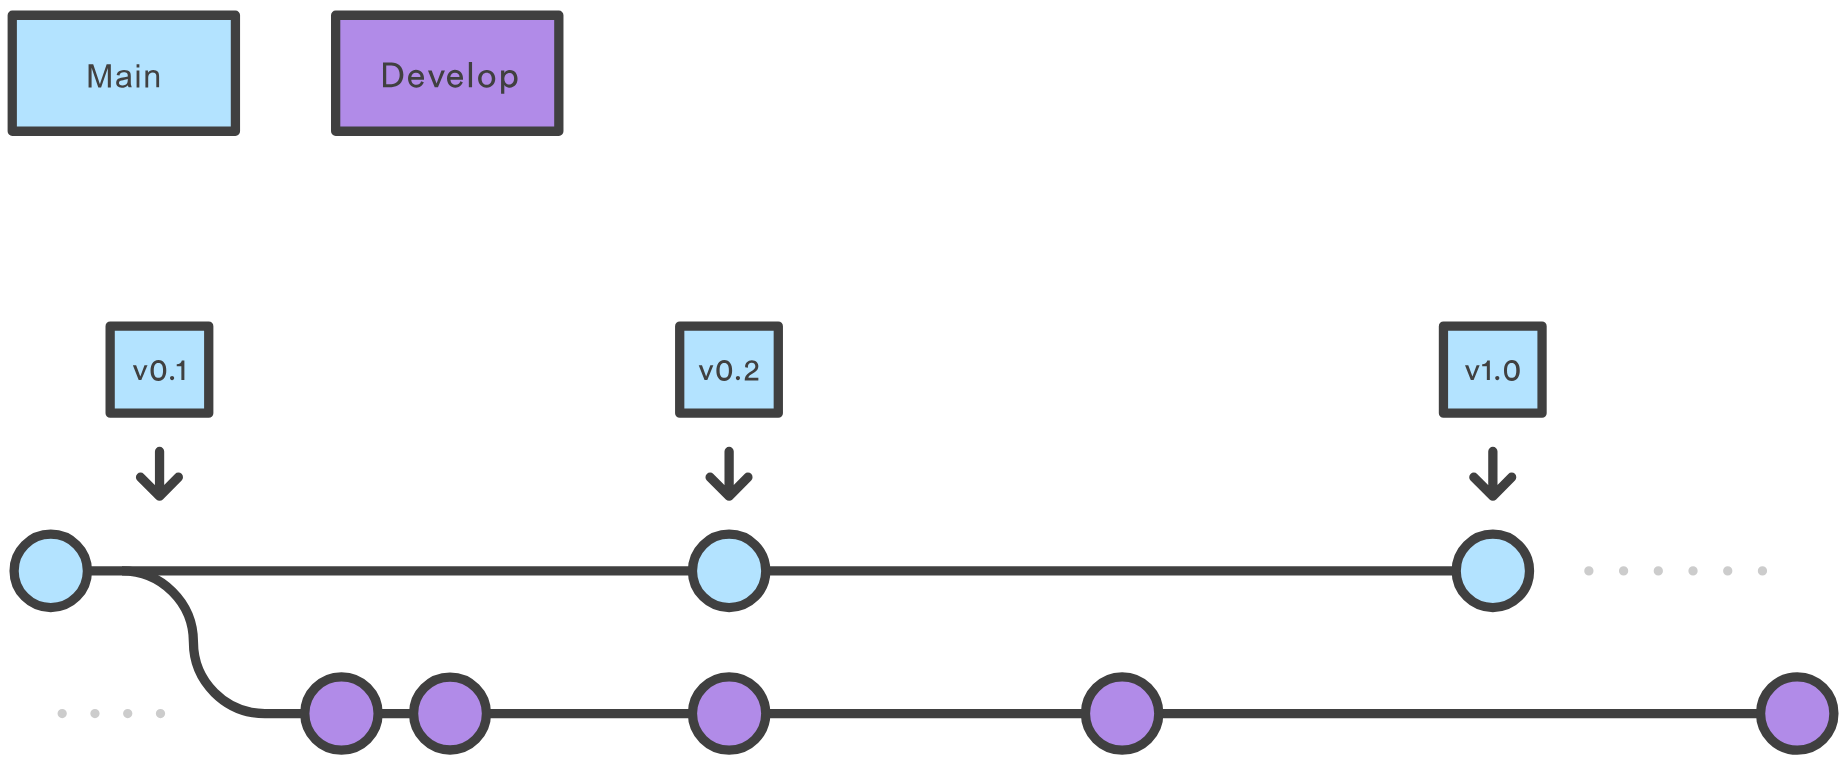
\includegraphics[width=.6\linewidth]{imagens/gitflow.png}
  \par
  \footnotesize{Fonte:TROCAR.}
\end{figure}

\section{Estrutura do documento}

\begin{itemize}
    \item \textbf{Capítulo 2 -- A empresa:} Esse Capítulo introduz a empresa e o processo organizacional.
    \item \textbf{Capítulo 3 -- Fundamentação teórica:} Esse Capítulo traz os fundamentos das teorias, conceitos e tecnologias utilizados durante o projeto.
    \item \textbf{Capítulo 4 -- Arquitetura e requisitos:} Esse Capítulo traz toda arquitetura e componentes da base do projeto. Assim como, os requisitos para a validação.
    \item \textbf{Capítulo 5 -- Desenvolvimento:} Esse Capítulo traz toda a estruturação do problema, e o desenvolvimento de análises, explicando o por quê de cada escolha durante o projeto.
    \item \textbf{Capítulo 6 -- Resultados e análises:} Esse Capítulo valida os passos tomados para garantir o sucesso do projeto. 
    \item \textbf{Capítulo 7 -- Conclusão e trabalhos futuros:} Esse Capítulo recapitula todos os processos e traz sugestões para novas funcionalidades do projeto.
\end{itemize}
